% =====================================================================
%  Review: tectonic significance of river-profile and drainage-basin
%  morphometry in low-strain NW Europe (Ardenne, western Rhenish shield,
%  northern Upper Rhine Graben).
%  Layout: A4, two columns, Palatino text, sans-serif headings,
%  numbered sections, Harvard (author--year) references.
%  All figures are redrawn from values published in the reviewed papers.
%  Compile: pdflatex main.tex  (run twice)
% =====================================================================
\documentclass[10pt,a4paper,twocolumn]{article}

% ---------------- Author details (edit before submission) ------------
\newcommand{\AuthorOne}{First Author}
\newcommand{\AuthorTwo}{Second Author}
\newcommand{\AffilOne}{Department of Geology, Name of University, City -- PIN, India}
\newcommand{\AffilTwo}{Department / Institute, Name of University, City -- PIN, India}
\newcommand{\CorrEmail}{corresponding.author@example.com}
\newcommand{\RunningTitle}{Tectonic significance of fluvial morphometry in NW Europe: a review}

% ---------------- Packages -------------------------------------------
\usepackage[T1]{fontenc}
\usepackage[utf8]{inputenc}
\usepackage{mathpazo}
\usepackage[scaled=0.92]{helvet}
\usepackage[a4paper,top=2.2cm,bottom=2.2cm,left=1.7cm,right=1.7cm,
            columnsep=0.7cm,headheight=14pt,headsep=0.4cm]{geometry}
\usepackage{amsmath}
\usepackage{booktabs,tabularx,array,multirow}
\usepackage[font=small,labelfont={bf,sf},labelsep=period,skip=4pt]{caption}
\usepackage{titlesec}
\usepackage{fancyhdr}
\usepackage[round,authoryear]{natbib}
\usepackage{xcolor}
\usepackage{tikz}
\usetikzlibrary{arrows.meta,positioning,calc,fit,backgrounds}
\usepackage{pgfplots}
\pgfplotsset{compat=1.16}
\usepgfplotslibrary{groupplots,fillbetween}
\usepackage{enumitem}
\usepackage{microtype}
\usepackage{xurl}
\usepackage[colorlinks=true,linkcolor=accent,citecolor=accent,urlcolor=accent]{hyperref}
\urlstyle{same}

% ---------------- Colours (colour-blind safe) -------------------------
\definecolor{accent}{RGB}{0,82,140}
\definecolor{boxgray}{RGB}{238,241,245}
\definecolor{cA}{RGB}{0,114,178}     % blue
\definecolor{cB}{RGB}{213,94,0}      % vermilion
\definecolor{cC}{RGB}{0,158,115}     % green
\definecolor{cD}{RGB}{204,121,167}   % purple
\definecolor{cE}{RGB}{90,90,90}      % grey

% ---------------- House style ------------------------------------------
\titleformat{\section}{\normalfont\sffamily\bfseries\large\color{accent}}{\thesection.}{0.5em}{}
\titleformat{\subsection}{\normalfont\itshape\normalsize}{\thesubsection.}{0.5em}{}
\titlespacing*{\section}{0pt}{11pt plus 2pt minus 1pt}{5pt}
\titlespacing*{\subsection}{0pt}{8pt plus 2pt}{3pt}
\setlength{\parindent}{1.1em}
\renewcommand{\arraystretch}{1.15}
\setlist{itemsep=1pt,topsep=3pt,leftmargin=1.3em}
\renewcommand{\topfraction}{0.9}
\renewcommand{\dbltopfraction}{0.9}
\renewcommand{\textfraction}{0.08}
\renewcommand{\floatpagefraction}{0.8}
\renewcommand{\dblfloatpagefraction}{0.8}

\pagestyle{fancy}
\fancyhf{}
\fancyhead[L]{\footnotesize\sffamily \AuthorOne{} and \AuthorTwo}
\fancyhead[R]{\footnotesize\sffamily\itshape \RunningTitle}
\fancyfoot[C]{\footnotesize\sffamily\thepage}
\renewcommand{\headrulewidth}{0.4pt}
\fancypagestyle{first}{\fancyhf{}%
  \fancyhead[L]{\footnotesize\sffamily\bfseries\color{accent} REVIEW ARTICLE}%
  \fancyhead[R]{\footnotesize\sffamily Tectonic geomorphology}%
  \fancyfoot[C]{\footnotesize\sffamily\thepage}}

\newcolumntype{L}{>{\raggedright\arraybackslash}X}
\newcolumntype{P}[1]{>{\raggedright\arraybackslash}p{#1}}
\newcommand{\kmsq}{km\textsuperscript{2}}
\newcommand{\permil}{\textperthousand}
\newcommand{\Hb}{\ensuremath{\int\!H_\mathrm{b}}}
\newcommand{\Hn}{\ensuremath{\int\!H_\mathrm{n}}}
\newcommand{\Hr}{\ensuremath{\int\!H_\mathrm{r}}}
\newcommand{\Hvm}{\ensuremath{H_\mathrm{vm}}}

% =====================================================================
\begin{document}
\twocolumn[{%
\thispagestyle{first}
\begin{center}
{\sffamily\bfseries\fontsize{15.5}{19}\selectfont\color{accent}
Testing the tectonic significance of river-profile and drainage-basin morphometry in
low-strain intraplate settings: a comparative review from the Ardenne, the western Rhenish
shield and the Upper Rhine Graben (NW Europe)\par}
\vspace{8pt}
{\large \AuthorOne\textsuperscript{a,*} and \AuthorTwo\textsuperscript{b}\par}
\vspace{4pt}
{\footnotesize\itshape \textsuperscript{a}\AffilOne\quad
\textsuperscript{b}\AffilTwo\\ \textsuperscript{*}Corresponding author. E-mail: \CorrEmail\par}
\end{center}
\vspace{4pt}
\noindent\rule{\textwidth}{0.6pt}\\[-2pt]
\noindent
\begin{minipage}[t]{0.29\textwidth}
\vspace{4pt}
{\sffamily\bfseries\footnotesize\color{accent} A R T I C L E \quad I N F O}\par
\vspace{2pt}\rule{\linewidth}{0.3pt}\par\vspace{3pt}
{\footnotesize\itshape Keywords:}\par
{\footnotesize Longitudinal river profile\\ Stream-gradient index\\ Mountain-front sinuosity\\
Hypsometric integral\\ $R_1$ and $S_\mathrm{r}$ indices\\ Intraplate uplift\\ Ardenne--Rhenish shield\\
Upper Rhine Graben\par}
\vspace{6pt}
{\footnotesize\itshape Highlights:}\par
{\footnotesize
\begin{itemize}[leftmargin=0.9em,itemsep=0pt,topsep=1pt]
  \item Three NW European studies of fluvial morphometry are compared.
  \item All three remove a dominant non-tectonic control before reading tectonics.
  \item Profile indices map where uplift acts; basin-scale ratios estimate when.
  \item The NE Ardenne--N Eifel stands out as the youngest uplift in two studies.
  \item An integrated, multi-scale workflow is proposed.
\end{itemize}\par}
\end{minipage}\hfill
\begin{minipage}[t]{0.67\textwidth}
\vspace{4pt}
{\sffamily\bfseries\footnotesize\color{accent} A B S T R A C T}\par
\vspace{2pt}\rule{\linewidth}{0.3pt}\par\vspace{3pt}
\small
Rivers in slowly deforming regions carry only faint traces of tectonics, and these traces are
easily confused with the effects of rock strength, discharge, inherited relief and Pleistocene
climate. This review compares three studies that tested how far morphometric indices can isolate a
tectonic signal in NW Europe. \citet{Demoulin1998} analysed the long profiles of 24 rivers in the
Ardenne using map-based measures of gradient, concavity and valley-side height.
\citet{PetersVanBalen2007} combined palaeogeographic reconstruction, fault--drainage overlays and
four geomorphic indices along the borders of the northern Upper Rhine Graben.
\citet{Demoulin2011} built a new index, $R_1$, from the hypsometric integrals of the basin, its
drainage network and its trunk stream for 85 rivers of the western Rhenish shield. Re-plotting their
published data shows a common strategy: each study first removes the dominant non-tectonic control
(hydrodynamics, lithology or basin size) and then interprets what remains. Mean river gradient in the
uplifted NE Ardenne (12.4\permil) is two to three times that of the western massif and the
forelands. Active and inactive segments of the graben border faults separate clearly in the joint
behaviour of mountain-front sinuosity (1.1--2.1) and valley shape (1.5--19.9). The slope $S_\mathrm{r}$ of
$R_1$ against the logarithm of basin area falls from 0.51 to 0.24 from the youngest to the oldest uplift
area. Profile indices therefore show where tectonics acts over $10^4$--$10^5$ years, whereas $S_\mathrm{r}$
gives the relative timing of uplift over $10^5$--$10^6$ years. We discuss the shared limits of these
methods (lithology, inheritance, data resolution and the lack of absolute ages) and propose a
multi-scale workflow for low-strain settings.
\end{minipage}\\[4pt]
\noindent\rule{\textwidth}{0.6pt}
\vspace{10pt}
}]

% =====================================================================
\section{Introduction}

Rivers respond to uplift and faulting by changing their slope, their long-profile shape and the
depth of their valleys, and these changes can be measured from maps and elevation models. Since the
early work on stream gradients \citep{Hack1973} and on mountain fronts and valley shapes
\citep{BullMcFadden1977}, a large family of morphometric indices has been used to map active
tectonics \citep{KellerPinter2002,BurbankAnderson2001,KirbyWhipple2012}. Most of these tools were,
however, developed and calibrated in fast-deforming settings such as California, Taiwan or the Betic
Cordillera, where uplift rates reach millimetres per year and the tectonic signal is strong
\citep{MerrittsVincent1989,Silva2003,ElHamdouni2008}.

Intraplate NW Europe poses a harder problem. Quaternary uplift and subsidence rates there are
mostly between a few hundredths and a few tenths of a millimetre per year. The landscape has been
reshaped by repeated glacial--interglacial cycles, it contains planation surfaces inherited from the
Tertiary, and the bedrock varies from soft marls to quartzites. Under these conditions, a change in
river gradient or valley shape may reflect lithology, a change in discharge or sediment load, a river
capture or a periglacial base-level fall just as easily as fault movement. The central question is
therefore not only whether tectonics is recorded in the landscape, but whether its record can be
separated from everything else.

Three studies from the Ardenne, the western Rhenish shield and the northern Upper Rhine Graben
(URG) approach this question from different directions. \citet{Demoulin1998} tested a set of
long-profile parameters on 24 rivers of the Ardenne, using only data from 1:25,000 topographic maps.
\citet{PetersVanBalen2007} examined how faulting has shaped the relief and drainage of the northern URG
through a palaeogeographic synthesis, an overlay of faults and drainage, and four geomorphic indices.
\citet{Demoulin2011} designed a composite index, $R_1$, that combines the hypsometric integrals of
basin, drainage network and trunk stream, and showed that the slope of its relation with basin size
records the relative age of uplift.

Taken together, the three papers cover more than a decade of methodological development and three
neighbouring structural settings: a Variscan massif undergoing broad uplift, an active rift with
well-mapped faults, and the wider Rhenish shield. No synthesis of these studies is available. This
review aims to (i) compare their settings, data and indices; (ii) bring their main results together,
using the published values to redraw key relationships; (iii) identify the common logic and the
shared limits of their methods; and (iv) propose a workflow for future work in low-strain regions.

% =====================================================================
\section{Scope and approach of the review}

The three papers were read in full and compared under five headings: tectonic setting, data and
resolution, indices and statistical treatment, main results, and stated limitations. All figures in
this review are new drawings based on numbers given in the tables and text of the original papers;
no published figure is reproduced. As a check on transcription, the 24 river gradients and bedload
proxies listed by \citet{Demoulin1998} were refitted: they return the published regression (gradient
$=7.467\,x-0.017$) and correlation coefficient ($r=0.83$) exactly. Values that we calculated, such as
ratios between regional means, are labelled as derived.

% =====================================================================
\section{Tectonic and geomorphic setting}

\begin{figure}[t]
\centering
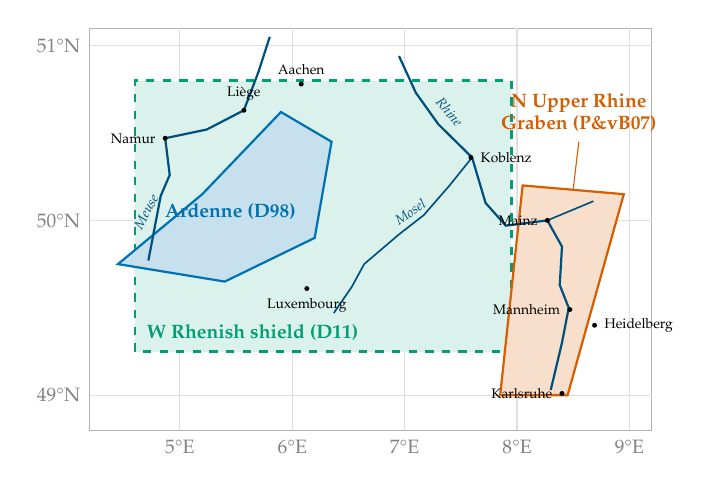
\begin{tikzpicture}[x=2.22cm*0.643,y=2.22cm,font=\scriptsize]
  % frame and graticule
  \draw[gray!60] (4.2,48.8) rectangle (9.2,51.1);
  \foreach \lo in {5,6,7,8,9}{\draw[gray!25] (\lo,48.8)--(\lo,51.1);
     \node[below,gray] at (\lo,48.8) {\lo\textdegree E};}
  \foreach \la in {49,50,51}{\draw[gray!25] (4.2,\la)--(9.2,\la);
     \node[left,gray] at (4.2,\la) {\la\textdegree N};}
  % study areas
  \fill[cC!14] (4.6,49.25) rectangle (7.95,50.8);
  \draw[cC,thick,dashed] (4.6,49.25) rectangle (7.95,50.8);
  \node[cC,anchor=south west,font=\scriptsize\bfseries] at (4.62,49.26) {W Rhenish shield (D11)};
  \fill[cA!22] (4.45,49.75)--(5.2,50.15)--(5.9,50.62)--(6.35,50.45)--(6.2,49.9)--(5.4,49.65)--cycle;
  \draw[cA,thick] (4.45,49.75)--(5.2,50.15)--(5.9,50.62)--(6.35,50.45)--(6.2,49.9)--(5.4,49.65)--cycle;
  \node[cA,font=\scriptsize\bfseries] at (5.45,50.05) {Ardenne (D98)};
  \fill[cB!20] (7.85,49.0)--(8.45,49.0)--(8.95,50.15)--(8.05,50.2)--cycle;
  \draw[cB,thick] (7.85,49.0)--(8.45,49.0)--(8.95,50.15)--(8.05,50.2)--cycle;
  \node[cB,font=\scriptsize\bfseries,align=center] at (8.55,50.62) {N Upper Rhine\\Graben (P\&vB07)};
  \draw[cB,thin] (8.55,50.45)--(8.5,50.18);
  % rivers (simplified)
  \draw[cA!70!black,line width=0.8pt] (4.72,49.77)--(4.83,50.14)--(4.91,50.26)--(4.87,50.47)--(5.24,50.52)--(5.57,50.63)--(5.70,50.85)--(5.80,51.05);
  \draw[cA!70!black,line width=0.8pt] (8.30,49.03)--(8.40,49.30)--(8.46,49.50)--(8.38,49.63)--(8.40,49.85)--(8.27,50.00)--(7.90,49.97)--(7.72,50.10)--(7.60,50.36)--(7.30,50.55)--(7.10,50.73)--(6.95,50.94);
  \draw[cA!70!black,line width=0.6pt] (6.37,49.47)--(6.53,49.62)--(6.64,49.75)--(6.95,49.92)--(7.17,50.03)--(7.40,50.20)--(7.60,50.36);
  \draw[cA!70!black,line width=0.6pt] (8.68,50.11)--(8.27,50.00);
  \node[cA!70!black,font=\tiny\itshape,rotate=62] at (4.70,50.05) {Meuse};
  \node[cA!70!black,font=\tiny\itshape,rotate=-50] at (7.40,50.62) {Rhine};
  \node[cA!70!black,font=\tiny\itshape,rotate=35] at (7.05,50.05) {Mosel};
  % towns
  \foreach \x/\y/\n/\p in {4.87/50.47/Namur/left,5.57/50.63/Li\`ege/above,6.13/49.61/Luxembourg/below,
      7.59/50.36/Koblenz/right,8.27/50.00/Mainz/left,8.47/49.49/Mannheim/left,8.40/49.01/Karlsruhe/left,
      8.69/49.40/Heidelberg/right,6.08/50.78/Aachen/above}
     {\fill (\x,\y) circle (0.9pt); \node[\p,font=\tiny] at (\x,\y) {\n};}
\end{tikzpicture}
\caption{Schematic location of the three study areas (boundaries simplified from the maps in the
original papers; rivers generalised). D98: \citet{Demoulin1998}; P\&vB07:
\citet{PetersVanBalen2007}; D11: \citet{Demoulin2011}.}
\label{fig:map}
\end{figure}

\subsection{Ardenne massif}

The Ardenne is a Palaeozoic massif belonging to the external Variscan belt and forms the western end
of the Rhenish shield (Fig.~\ref{fig:map}). Its basement is cut by ENE--WSW folds and thrusts and by
younger NW--SE to NNW--SSE faults, which produces strong contrasts in rock resistance over short
distances \citep{Demoulin1998}. Oligocene marine sands now lying at about 700~m on the Hautes Fagnes
plateau show at least 400--500~m of uplift of the NE Ardenne since the Oligocene, against less than
200~m in the west. The Quaternary uplift rate is estimated at about 0.1~mm\,a$^{-1}$ in the NE and no
more than 0.025~mm\,a$^{-1}$ in the west and south. Some NNW--SSE faults linked to the Lower Rhine rift
moved by up to 7~m in the last 100~ka, and the area has a moderate seismicity with one historical
event of about $M_\mathrm{L}$\,6 \citep{Demoulin1998}. Annual rainfall ranges from about
800~mm in the forelands to more than 1400~mm on the highest summits.

\subsection{Western Rhenish shield}

The study area of \citet{Demoulin2011} covers about $240\times170$~\kmsq{} west of the Rhine, from the
Ardennes and Eifel in the north to the Hunsrück, the Saar--Nahe basin and the Palatinate in the south.
The bedrock is largely slaty and of fairly uniform erodibility. Deformed Tertiary planation surfaces
indicate about 450~m of rock uplift since the Oligocene. Fluvial terraces show that uplift accelerated
in two steps during the Quaternary, peaking at about 0.5~mm\,a$^{-1}$ in the NE Ardennes and Eifel
between about 0.73 and 0.4~Ma \citep{VanBalen2000,DemoulinHallot2009}. An uplift wave appears to
have moved northwards across the massif since the early Pleistocene, towards the northern Ardennes and
Eifel, where uplift is strongest today \citep{DemoulinHallot2009}. This allowed three sub-areas of
different uplift age to be defined (Section~\ref{sec:wrs}).

\subsection{Northern Upper Rhine Graben}

The URG is the central segment of the European Cenozoic Rift System. Its main rifting phase took place
in the Oligocene and Miocene, and subsidence has continued at a lower rate since then
\citep{PetersVanBalen2007}. Quaternary sediments reach about 380~m in the Heidelberger Loch next to the
Eastern Border Fault, where subsidence peaked at about 0.2~mm\,a$^{-1}$; elsewhere rates are about an
order of magnitude lower. An average deformation rate of 0.03~mm\,a$^{-1}$ means that one metre of
relief takes about 30~ka to build, a span long enough for erosion to remove it. The western graben
shoulder has been uplifted relative to the subsiding east, and the valley floor has been heavily
modified by human activity. Unlike the two massifs, the URG therefore combines well-mapped faults
with very slow, localised deformation.

\begin{table*}[t]
\centering
\caption{Profile of the three reviewed studies.}
\label{tab:profile}
\footnotesize
\begin{tabularx}{\textwidth}{@{}P{2.6cm}LLL@{}}
\toprule
& \textbf{\citet{Demoulin1998}} & \textbf{\citet{PetersVanBalen2007}} & \textbf{\citet{Demoulin2011}}\\
\midrule
Journal & \textit{Geomorphology} 24 & \textit{Global and Planetary Change} 58 & \textit{Geomorphology} 126\\
Area & Ardenne massif and forelands (Meuse basin) & Northern Upper Rhine Graben and shoulders & Western Rhenish shield (Ardennes to Palatinate)\\
Tectonic style & Broad uplift, NE Ardenne strongest; minor faulting & Rift with border and intra-graben faults & En-bloc uplift migrating from S to N\\
Typical rates & $\le$0.025 to $\sim$0.1~mm\,a$^{-1}$ & 0.01--0.08 (mean 0.03)~mm\,a$^{-1}$ & up to $\sim$0.5~mm\,a$^{-1}$ (0.73--0.4~Ma)\\
Data & 1:25,000 maps, 2.5--5~m contours; 24 rivers, orders 3--5, 21--65~km & DGM50 (30~m) and DGM5 DEMs; fault and terrace maps; 20~m contour interval & SRTM 3$''$ DEM; 85 rivers, orders 2--6, $\sim$15--4000~\kmsq{}\\
Main indices & Gradient, $E_\mathrm{r}$, $H_\mathrm{max}$, $E_\mathrm{q}$, \Hvm, \Hvm$\cdot L/A$ & SL, S, $S_\mathrm{mf}$, $V_\mathrm{f}$, fault--drainage orientation & \Hb, \Hn, \Hr, $I_\mathrm{b}$, $I_\mathrm{r}$, $R_1$, $S_\mathrm{r}$\\
Statistics & Correlation, regression, K-means clustering & Regional means and ranges & Regression on $\ln A$, ANCOVA tests\\
Main question & Where are areas of differential vertical movement? & Which fault segments are active, and since when? & When did uplift affect each area, in relative terms?\\
\bottomrule
\end{tabularx}
\end{table*}

% =====================================================================
\section{Morphometric approaches compared}

Table~\ref{tab:profile} summarises the three studies and Table~\ref{tab:indices} defines their
indices. Fig.~\ref{fig:timescale} places the indices on an indicative time axis.

\subsection{Long-profile geometry and a bedload proxy (Ardenne)}

\citet{Demoulin1998} digitised 24 rivers of third to fifth order from 1:25,000 maps, using contour
crossings every 2.5 or 5~m. The digitised lengths matched field-levelled lengths to within 0.1\%
on average. Profiles were resampled every 200~m, smoothed and normalised, so that rivers of
different length and relief could be compared (Fig.~\ref{fig:concept}a). Three parameters describe
profile shape: $E_\mathrm{r}$, the area between the profile and a straight line joining source and
mouth, as a percentage of the triangle below that line; $H_\mathrm{max}$, the largest vertical gap
between profile and line; and $E_\mathrm{q}$, the normalised distance from the source at which this
gap occurs. A well-graded, strongly concave profile has a high $E_\mathrm{r}$ and $H_\mathrm{max}$
and a low $E_\mathrm{q}$.

The key methodological step was to estimate how much of the river gradient is simply explained by
hydraulics. Bankfull discharge in the region scales closely with basin area ($r=0.94$ for 40 rivers),
and the mean height of the valley sides, \Hvm, was proposed as a map-based proxy for bedload supply.
\Hvm\ correlated with the median bedload size at the river mouth ($r=0.79$, 18 rivers) but not along
individual rivers. The product $\Hvm\cdot L/A$, which expresses the total valley-side surface relative
to basin size, explained most of the variation in mean gradient (Fig.~\ref{fig:d98reg}). Rivers that
plot far from this regression were taken to be influenced by non-hydrodynamic factors, mainly
lithology or tectonics.

\subsection{Gradient, mountain-front and valley indices (Upper Rhine Graben)}

\citet{PetersVanBalen2007} first compiled a series of six palaeogeographic maps from the Late Miocene to
the present, based on earlier work and new terrace and fault mapping. They then compared the
orientations of 156 intra-graben and 94 shoulder fault segments with 412 stream segments to detect
structural control of drainage. Finally, they computed four indices from a 30~m DEM, using a finer
DEM along the Western Border Fault (WBF) scarp: the stream length--gradient index SL of
\citet{Hack1973}, with a 20~m contour interval; its first derivative S, which highlights where SL
changes most sharply; the mountain-front sinuosity $S_\mathrm{mf}$, over 15~km segments of the border
faults; and the valley-floor width-to-height ratio $V_\mathrm{f}$, measured 1~km upstream of the border
faults \citep{BullMcFadden1977}.

\subsection{Hypsometric integrals at three levels (western Rhenish shield)}

\citet{Demoulin2011} reasoned that a relative fall in base level reaches the landscape in three stages:
the trunk stream first, then the drainage network, and finally the hillslopes of the whole basin. Each
stage is described by an integral of a normalised elevation curve (Fig.~\ref{fig:concept}b): the
classic basin hypsometric integral \Hb\ \citep{Strahler1952}; \Hn, the same integral for the pixels of
the drainage network; and \Hr, the integral of the trunk-stream long profile scaled to the basin relief.
Differences between them measure how deeply the network is cut into the basin
($I_\mathrm{b}=\Hb-\Hn$) and how far incision has spread from the trunk into the network
($I_\mathrm{r}=\Hn-\Hr$). Their ratio, $R_1=I_\mathrm{r}/I_\mathrm{b}$, should cancel much of the
lithological effect, which acts on both terms. The indices were computed for 85 rivers from the SRTM
3$''$ DEM. Tests suggested that the coarse resolution changes $R_1$ by no more than a few per cent.

\subsection{Different data, different questions}

The three studies differ as much in their data as in their aims. The map-based analysis of 1998 used
contour intervals of 2.5--5~m, finer than either DEM-based study, but could only sample 24 rivers.
The URG study used a 30~m DEM with a 20~m contour interval, which its authors note may be too coarse to
detect small gradient changes on the low-gradient graben floor. The 2011 study accepted the
lowest resolution of the three in exchange for a nearly universal data source and a large sample of
basins. These choices follow from the questions asked: \textit{where} differential movement occurs
(1998), \textit{which} fault segments are active (2007), and \textit{when} uplift happened in relative
terms (2011).

\begin{table*}[t]
\centering
\caption{Morphometric indices used in the reviewed studies.}
\label{tab:indices}
\footnotesize
\begin{tabularx}{\textwidth}{@{}P{2.3cm}P{4.6cm}LP{2.0cm}@{}}
\toprule
\textbf{Index} & \textbf{Definition} & \textbf{Reading} & \textbf{Source}\\
\midrule
Mean gradient & Elevation drop over river length (\permil) & Higher where profiles are steep or not yet graded & D98\\
$E_\mathrm{r}$ & Area between profile and source--mouth line, \% of triangle & High: concave, graded; low or negative: straight or convex & D98\\
$H_\mathrm{max}$, $E_\mathrm{q}$ & Largest profile--line gap; its normalised distance from source & High $H_\mathrm{max}$, low $E_\mathrm{q}$: concavity migrated far upstream & D98\\
\Hvm, $\Hvm\!\cdot\!L/A$ & Mean valley-side height; times river length over basin area & Proxy for bedload/discharge ratio; residuals flag non-hydraulic controls & D98\\
SL & $(\Delta H/\Delta L)\cdot L$, where $L$ is measured upstream to the source & High: local steepening of the channel & \citet{Hack1973}; P\&vB07\\
S & $(\Delta\mathrm{slope}/\Delta L)\cdot L$ & Sign changes locate breaks in slope & P\&vB07\\
$S_\mathrm{mf}$ & $L_\mathrm{mf}/L_\mathrm{s}$: front length along the foot over straight length & $\approx$1: straight, fault-controlled front; $>$2: embayed, eroded front & \citet{BullMcFadden1977}; P\&vB07\\
$V_\mathrm{f}$ & $2V_\mathrm{fw}/[(E_\mathrm{ld}-E_\mathrm{sc})+(E_\mathrm{rd}-E_\mathrm{sc})]$ & Low: V-shaped valley, active incision; high: broad floor & \citet{BullMcFadden1977}; P\&vB07\\
\Hb, \Hn, \Hr & Integrals of normalised basin, network and trunk-profile curves & Long-, middle- and short-term response to base-level fall & D11\\
$I_\mathrm{b}$, $I_\mathrm{r}$ & $\Hb-\Hn$; $\Hn-\Hr$ & Incision of network into basin; spread of incision into network & D11\\
$R_1$, $S_\mathrm{r}$ & $R_1=I_\mathrm{r}/I_\mathrm{b}$; $S_\mathrm{r}$ = slope of $R_1=S_\mathrm{r}\ln A+b$ & $S_\mathrm{r}$ decreases with time since uplift & D11\\
\bottomrule
\end{tabularx}
\end{table*}

\begin{figure}[t]
\centering
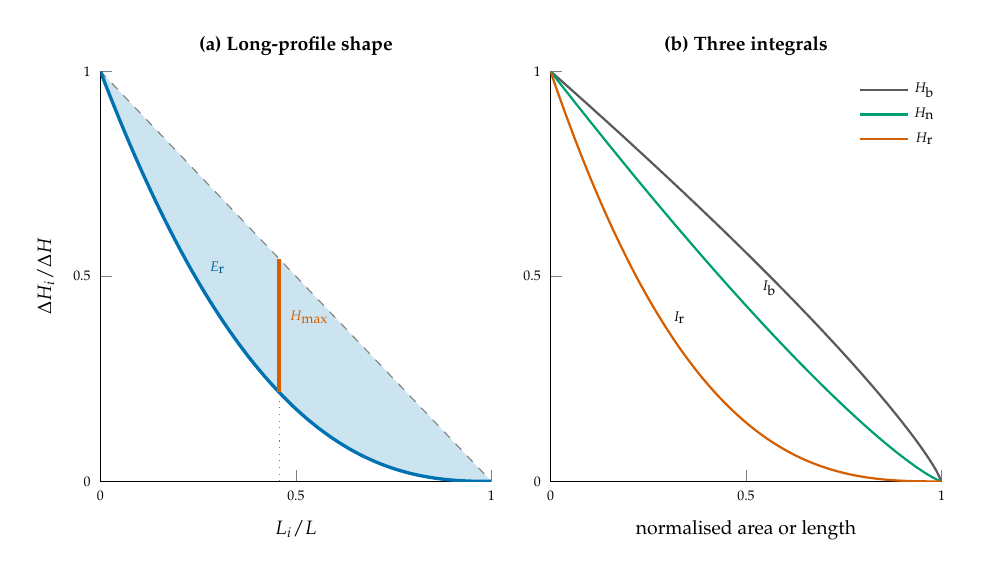
\begin{tikzpicture}
\begin{groupplot}[group style={group size=2 by 1,horizontal sep=0.75cm},
  width=0.54\columnwidth,height=0.56\columnwidth,
  xmin=0,xmax=1,ymin=0,ymax=1,tick label style={font=\tiny},
  label style={font=\scriptsize},title style={font=\scriptsize\bfseries,yshift=-4pt},
  axis lines*=left,xtick={0,0.5,1},ytick={0,0.5,1}]
\nextgroupplot[title={(a) Long-profile shape},xlabel={$L_i/L$},ylabel={$\Delta H_i/\Delta H$}]
  \addplot[name path=line,gray,dashed,domain=0:1] {1-x};
  \addplot[name path=prof,cA,very thick,domain=0:1,samples=80] {(1-x)^2.5};
  \addplot[cA!20] fill between[of=line and prof];
  \draw[cB,very thick] (axis cs:0.457,0.217) -- (axis cs:0.457,0.543);
  \node[cB,font=\tiny,right] at (axis cs:0.46,0.40) {$H_\mathrm{max}$};
  \draw[cB,dotted] (axis cs:0.457,0) -- (axis cs:0.457,0.217);
  \node[cB,font=\tiny,below] at (axis cs:0.457,0.0) {$E_\mathrm{q}$};
  \node[cA!80!black,font=\tiny] at (axis cs:0.30,0.52) {$E_\mathrm{r}$};
\nextgroupplot[title={(b) Three integrals},xlabel={normalised area or length},
  legend style={font=\tiny,draw=none,fill=none,at={(1.02,1.0)},anchor=north east}]
  \addplot[cE,thick,domain=0:1,samples=80] {(1-x)^0.842};
  \addplot[cC,thick,domain=0:1,samples=80] {(1-x)^1.222};
  \addplot[cB,thick,domain=0:1,samples=80] {(1-x)^2.80};
  \legend{$H_\mathrm{b}$,$H_\mathrm{n}$,$H_\mathrm{r}$}
  \node[font=\tiny] at (axis cs:0.56,0.47) {$I_\mathrm{b}$};
  \node[font=\tiny] at (axis cs:0.33,0.40) {$I_\mathrm{r}$};
\end{groupplot}
\end{tikzpicture}
\caption{Geometry of the profile and basin indices. (a) Idealised normalised long profile with the
parameters of \citet{Demoulin1998}. (b) Idealised curves with the same integrals as the Ahr basin
example of \citet{Demoulin2011} (\Hb\,=\,0.543, \Hn\,=\,0.450, \Hr\,=\,0.263, giving
$I_\mathrm{b}=0.093$, $I_\mathrm{r}=0.187$ and $R_1=2.01$).}
\label{fig:concept}
\end{figure}

\begin{figure*}[t]
\centering
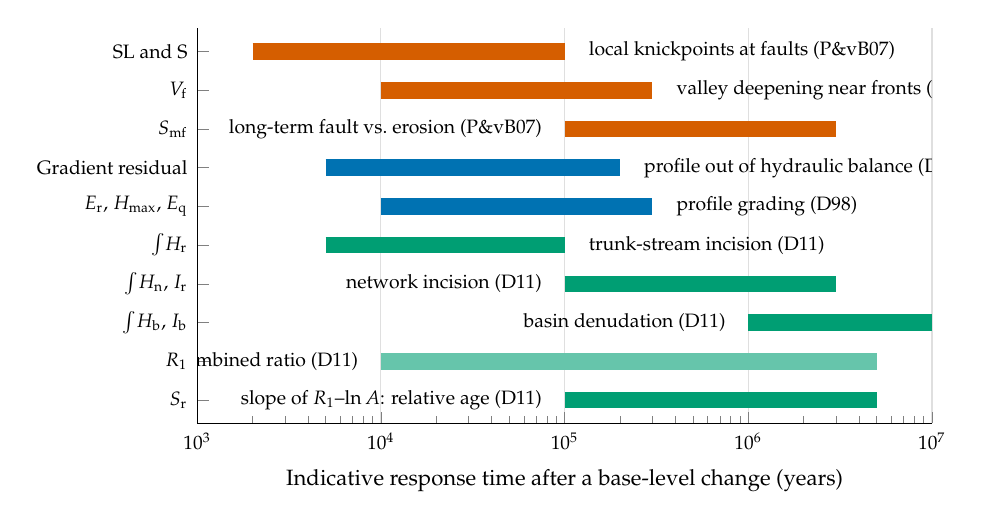
\begin{tikzpicture}[font=\footnotesize]
\begin{axis}[width=0.9\textwidth,height=6.6cm,xmode=log,xmin=1e3,xmax=1e7,
  ymin=0.4,ymax=10.6,ytick={1,...,10},
  yticklabels={SL and S,$V_\mathrm{f}$,$S_\mathrm{mf}$,Gradient residual,{$E_\mathrm{r}$, $H_\mathrm{max}$, $E_\mathrm{q}$},\Hr,{\Hn, $I_\mathrm{r}$},{\Hb, $I_\mathrm{b}$},$R_1$,$S_\mathrm{r}$},
  y dir=reverse,xlabel={Indicative response time after a base-level change (years)},
  xtick={1e3,1e4,1e5,1e6,1e7},axis lines*=left,xmajorgrids,grid style={gray!25},
  tick label style={font=\scriptsize}]
  % P&vB07 (vermilion), D98 (blue), D11 (green)
  \addplot[cB,line width=6pt] coordinates {(2e3,1) (1e5,1)};
  \addplot[cB,line width=6pt] coordinates {(1e4,2) (3e5,2)};
  \addplot[cB,line width=6pt] coordinates {(1e5,3) (3e6,3)};
  \addplot[cA,line width=6pt] coordinates {(5e3,4) (2e5,4)};
  \addplot[cA,line width=6pt] coordinates {(1e4,5) (3e5,5)};
  \addplot[cC,line width=6pt] coordinates {(5e3,6) (1e5,6)};
  \addplot[cC,line width=6pt] coordinates {(1e5,7) (3e6,7)};
  \addplot[cC,line width=6pt] coordinates {(1e6,8) (1e7,8)};
  \addplot[cC!60,line width=6pt] coordinates {(1e4,9) (5e6,9)};
  \addplot[cC,line width=6pt] coordinates {(1e5,10) (5e6,10)};
  \node[anchor=west,font=\scriptsize] at (axis cs:1.2e5,1) {local knickpoints at faults (P\&vB07)};
  \node[anchor=west,font=\scriptsize] at (axis cs:3.6e5,2) {valley deepening near fronts (P\&vB07)};
  \node[anchor=east,font=\scriptsize] at (axis cs:0.85e5,3) {long-term fault vs.\ erosion (P\&vB07)};
  \node[anchor=west,font=\scriptsize] at (axis cs:2.4e5,4) {profile out of hydraulic balance (D98)};
  \node[anchor=west,font=\scriptsize] at (axis cs:3.6e5,5) {profile grading (D98)};
  \node[anchor=west,font=\scriptsize] at (axis cs:1.2e5,6) {trunk-stream incision (D11)};
  \node[anchor=east,font=\scriptsize] at (axis cs:0.85e5,7) {network incision (D11)};
  \node[anchor=east,font=\scriptsize] at (axis cs:0.85e6,8) {basin denudation (D11)};
  \node[anchor=east,font=\scriptsize] at (axis cs:0.85e4,9) {combined ratio (D11)};
  \node[anchor=east,font=\scriptsize] at (axis cs:0.85e5,10) {slope of $R_1$--$\ln A$: relative age (D11)};
\end{axis}
\end{tikzpicture}
\caption{Indicative time windows during which each index reacts to a fall in base level, compiled from
the reasoning of the reviewed papers (colours: vermilion, \citealp{PetersVanBalen2007}; blue,
\citealp{Demoulin1998}; green, \citealp{Demoulin2011}). Ranges are qualitative and depend on basin size,
rock strength and uplift rate.}
\label{fig:timescale}
\end{figure*}

% =====================================================================
\section{Main findings}

\subsection{Ardenne: regional uplift and local subsidence from profile parameters}

\begin{table}[t]
\centering
\caption{Mean profile parameters by sub-region of the Ardenne (from \citealp{Demoulin1998}).}
\label{tab:d98}
\scriptsize
\setlength{\tabcolsep}{3.2pt}
\begin{tabular}{@{}lcccccc@{}}
\toprule
\textbf{Sub-region} & $n$ & \textbf{Grad.} & $E_\mathrm{r}$ & $H_\mathrm{max}$ & $E_\mathrm{q}$ & $\Hvm\!\cdot\!L/A$\\
& & (\permil) & (\%) & & & \\
\midrule
NE Ardenne & 6 & 12.4 & 17.8 & 0.17 & 0.36 & 1.51\\
Central Ardenne & 5 & 6.9 & 23.7 & 0.19 & 0.42 & 0.97\\
W Ardenne--Condroz & 7 & 6.1 & 13.2 & 0.13 & 0.39 & 0.90\\
N foreland & 3 & 4.4 & 25.0 & 0.23 & 0.27 & 0.51\\
S foreland & 3 & 4.1 & 45.9 & 0.36 & 0.23 & 0.66\\
\bottomrule
\end{tabular}
\end{table}

The regional means already show a clear pattern (Table~\ref{tab:d98}). Mean river gradient in the
uplifted NE Ardenne is twice that of the western massif and nearly three times that of the two
forelands (derived ratios 2.0 and 2.8--3.0). The southern foreland, a stable area with weak Mesozoic
rocks, has the most concave profiles ($E_\mathrm{r}$ 45.9\%).

\begin{figure}[t]
\centering
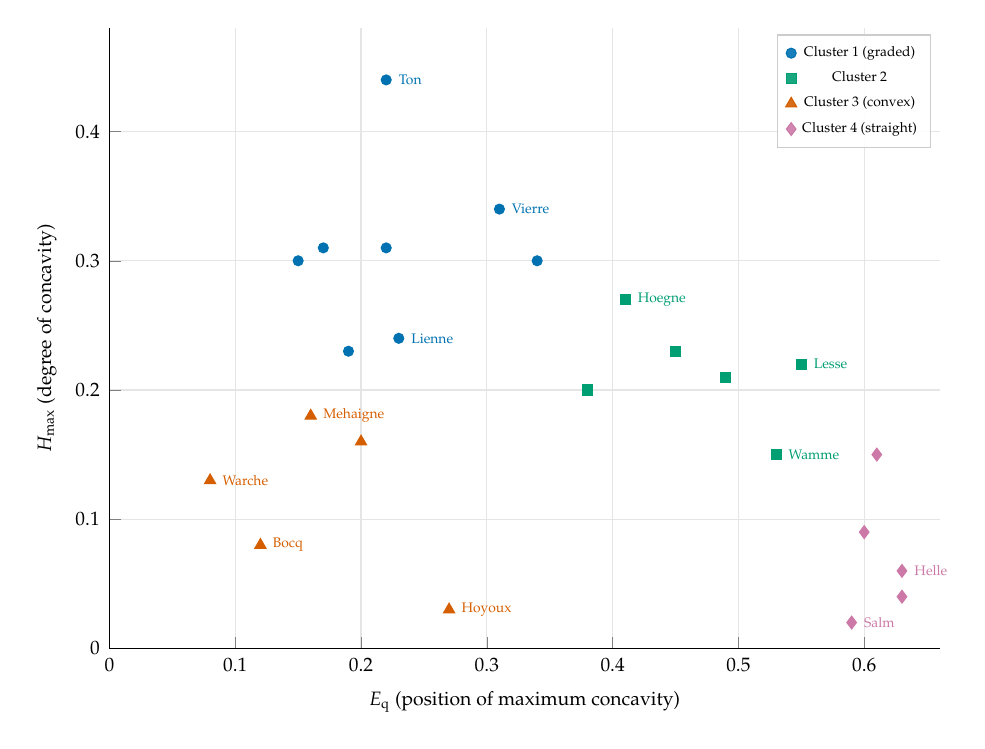
\begin{tikzpicture}
\begin{axis}[width=\columnwidth,height=0.78\columnwidth,
  xmin=0,xmax=0.66,ymin=0,ymax=0.48,
  xlabel={$E_\mathrm{q}$ (position of maximum concavity)},
  ylabel={$H_\mathrm{max}$ (degree of concavity)},
  label style={font=\scriptsize},tick label style={font=\scriptsize},
  axis lines*=left,grid=major,grid style={gray!20},
  legend style={font=\tiny,at={(0.99,0.99)},anchor=north east,draw=gray!40,fill=white,fill opacity=0.9,text opacity=1},
  nodes near coords,point meta=explicit symbolic,
  every node near coord/.append style={font=\tiny,anchor=west,xshift=1pt}]
\addplot[only marks,mark=*,cA,mark size=1.8pt] coordinates {
  (0.31,0.34)[Vierre] (0.17,0.31)[] (0.22,0.44)[Ton] (0.15,0.30)[]
  (0.34,0.30)[] (0.19,0.23)[] (0.22,0.31)[] (0.23,0.24)[Lienne]};
\addplot[only marks,mark=square*,cC,mark size=1.8pt] coordinates {
  (0.55,0.22)[Lesse] (0.45,0.23)[] (0.53,0.15)[Wamme] (0.38,0.20)[] (0.49,0.21)[] (0.41,0.27)[Hoegne]};
\addplot[only marks,mark=triangle*,cB,mark size=2.3pt] coordinates {
  (0.16,0.18)[Mehaigne] (0.12,0.08)[Bocq] (0.27,0.03)[Hoyoux] (0.08,0.13)[Warche] (0.20,0.16)[]};
\addplot[only marks,mark=diamond*,cD,mark size=2.3pt] coordinates {
  (0.63,0.06)[Helle] (0.59,0.02)[Salm] (0.63,0.04)[] (0.60,0.09)[] (0.61,0.15)[]};
\legend{Cluster 1 (graded),Cluster 2,Cluster 3 (convex),Cluster 4 (straight)}
\end{axis}
\end{tikzpicture}
\caption{Concavity ($H_\mathrm{max}$) against position of maximum concavity ($E_\mathrm{q}$) for the
24 Ardenne rivers, grouped by the K-means clusters of \citet{Demoulin1998}. Redrawn from the values in
his Tables 1 and 4; only some points are labelled.}
\label{fig:d98clu}
\end{figure}

\begin{figure}[t]
\centering
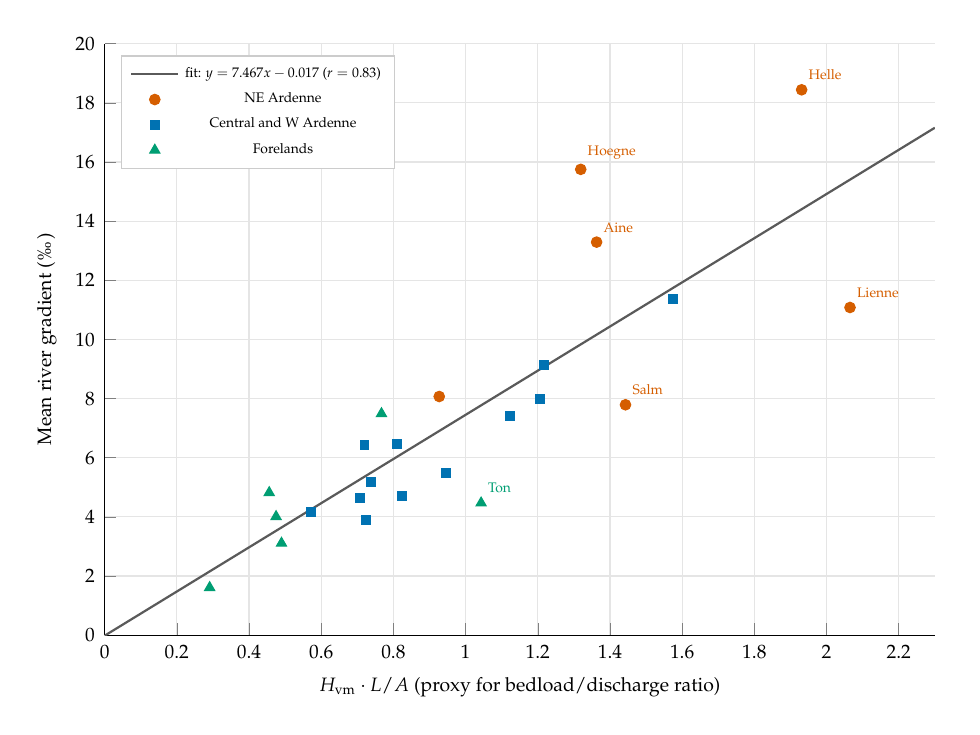
\begin{tikzpicture}
\begin{axis}[width=\columnwidth,height=0.75\columnwidth,
  xmin=0,xmax=2.3,ymin=0,ymax=20,
  xlabel={$\Hvm\cdot L/A$ (proxy for bedload/discharge ratio)},
  ylabel={Mean river gradient (\permil)},
  label style={font=\scriptsize},tick label style={font=\scriptsize},
  axis lines*=left,grid=major,grid style={gray!20},
  legend style={font=\tiny,at={(0.02,0.98)},anchor=north west,draw=gray!40},
  nodes near coords,point meta=explicit symbolic,
  every node near coord/.append style={font=\tiny,anchor=south west,xshift=-1pt}]
\addplot[cE,thick,domain=0:2.3] {7.467*x-0.017};
\addplot[only marks,mark=*,cB,mark size=1.9pt] coordinates {
  (1.319,15.75)[Hoegne] (1.931,18.44)[Helle] (0.927,8.07)[] (1.443,7.79)[Salm] (2.065,11.08)[Lienne] (1.363,13.29)[Aine]};
\addplot[only marks,mark=square*,cA,mark size=1.6pt] coordinates {
  (0.945,5.47)[] (0.824,4.70)[] (0.72,6.42)[] (0.81,6.48)[] (1.574,11.36)[]
  (0.739,5.17)[] (0.571,4.16)[] (0.723,3.90)[] (1.206,7.98)[] (0.708,4.65)[] (1.216,9.14)[] (1.122,7.42)[]};
\addplot[only marks,mark=triangle*,cC,mark size=2.1pt] coordinates {
  (0.767,7.49)[] (0.291,1.61)[] (0.475,4.01)[] (0.49,3.11)[] (0.456,4.82)[] (1.043,4.47)[Ton]};
\legend{fit: $y=7.467x-0.017$ ($r=0.83$),NE Ardenne,Central and W Ardenne,Forelands}
\end{axis}
\end{tikzpicture}
\caption{Mean gradient against the bedload/discharge proxy for the 24 rivers of
\citet{Demoulin1998}, redrawn from his Table 1. Points above the line (Hoegne, Helle, Aine) are steeper
than hydraulics alone explains; points below (Lienne, Salm, Ton) are more deeply incised.}
\label{fig:d98reg}
\end{figure}

Profile shape gives a finer picture. Clustering on $H_\mathrm{max}$ and $E_\mathrm{q}$ alone produced four
recognisable profile types (Fig.~\ref{fig:d98clu}). Cluster~1 holds well-graded, concave profiles,
mostly outside the massif. Cluster~2 groups the slightly less concave rivers of west-central Ardenne.
Cluster~3 holds rivers with a convex lower course, and cluster~4 rivers with nearly straight profiles.
For the Hoyoux, Samson and Bocq, which flow to the Meuse between Dinant and Huy, neither lithology nor
hydrology explains the convexity, and the Meuse itself has not incised there for about 100~ka.
\citet{Demoulin1998} therefore inferred subsidence of the Namur area relative to the Condroz, which
agrees with repeated levelling surveys from 1948--1978. Straight profiles of the Helle and Salm, by
contrast, reflect resistant bedrock combined with uplift of their NE Ardenne source areas.

The regression of gradient on $\Hvm\cdot L/A$ is the most informative single result
(Fig.~\ref{fig:d98reg}). Except for the Ton, a sand-bed river on erodible rock, all outliers lie in the NE
Ardenne. The Hoegne, Helle and Aine are steeper than their hydraulic setting predicts, which points to
delayed grading under current uplift. The Lienne and Salm are less steep than predicted, which
suggests strong incision in response to an earlier phase of uplift. Knickpoints along the Lesse,
Lomme and Wamme point to a Late Pleistocene base-level fall in the Famenne, which could be either
periglacial or tectonic.

Two cautions run through the study. First, the clusters do not follow the tectonic sub-units neatly:
rivers of the NE and W Ardenne fall into all four groups, and the very different profiles of
neighbouring NE Ardenne rivers remained unexplained. Second, some contrasts are inherited rather than
active. The difference between Ardenne and Condroz rivers reflects an Oligocene planation surface cut
more than 100~m below the Ardenne surfaces, not present-day movement.

\subsection{Northern Upper Rhine Graben: segmented border faults and a preserved tectonic landscape}

The palaeogeographic synthesis shows that uplift of the western graben shoulder shaped the Rhine and
its terraces throughout the Pleistocene. Offset terraces give deformation rates of
0.01--0.08~mm\,a$^{-1}$ for the Early--Middle Pleistocene and about 0.03~mm\,a$^{-1}$ for the Late
Pleistocene, so the rate has stayed low and fairly constant \citep{PetersVanBalen2007}. Faults with
a morphological expression mostly strike NNE, parallel to the graben. Several of them coincide with
terrace scarps, which the authors interpret as composite scarps of fluvial and tectonic origin.
NW--SE faults appear to guide some streams in the eastern graben. Linear ENE--WSW scarps in the
Vorderpfalz do not follow any known fault and were judged to be purely erosional.

\begin{table*}[t]
\centering
\caption{Regional means of the geomorphic indices of the northern URG (from \citealp{PetersVanBalen2007},
their Table 1), with the interpretation given in that study.}
\label{tab:pvb}
\footnotesize
\begin{tabularx}{\textwidth}{@{}lcccccccL@{}}
\toprule
\textbf{Region} & \textbf{$|$S$|$} & \textbf{SL} & \textbf{SL near fault} & \textbf{$V_\mathrm{f}$ mean} & \textbf{$V_\mathrm{f}$ range} & \textbf{$S_\mathrm{mf}$ mean} & \textbf{$S_\mathrm{mf}$ range} & \textbf{Interpretation}\\
\midrule
\multicolumn{9}{@{}l}{\textit{Eastern graben shoulder}}\\
Kraichgau & 1.4 & 36 & 34--79 & 13.6 & 4.1--31.3 & 2.1 & 1.8--2.4 & Erosion dominant; graded streams\\
Odenwald & 12.0 & 94 & 170--271 & 1.9 & 0.3--5.6 & 1.6 & 1.2--3.0 & Tectonic in south; front shaped by strong rock\\
Sprendlinger Horst & 0.4 & 31 & 16--33 & 19.9 & 14.7--27 & 1.9 & 1.5--2.5 & Erosion dominant\\
\multicolumn{9}{@{}l}{\textit{Western graben shoulder}}\\
WBF scarp & 8.1 & 76 & 170--302 & 5.1 & 3.4--11.0 & 1.1 & 1.1--1.2 & Tectonic and fluvial (composite scarp)\\
Rheinhess.\ Hügelland & 7.8 & 74 & 71--101 & 2.4 & 1.1--4.6 & 1.4 & 1.1--1.8 & Erosion and uplift in balance\\
N Pfälzer Wald & 13.4 & 102 & 180--442 & 1.5 & 0.6--4.0 & 1.4 & 1.2--1.9 & Active uplift\\
S Pfälzer Wald & 1.3 & 52 & 49--100 & 2.1 & 0.7--3.5 & 2.0 & 1.7--2.3 & Erosion dominant\\
\multicolumn{9}{@{}l}{\textit{Northwestern regions}}\\
Rhenish Massif & 13.0 & 136 & -- & -- & -- & -- & -- & Gradients reflect resistant rock\\
Mainz Basin & 2.6 & 63 & -- & -- & -- & -- & -- & Soft rocks, gentle slopes\\
\bottomrule
\end{tabularx}
\end{table*}

\begin{figure}[t]
\centering
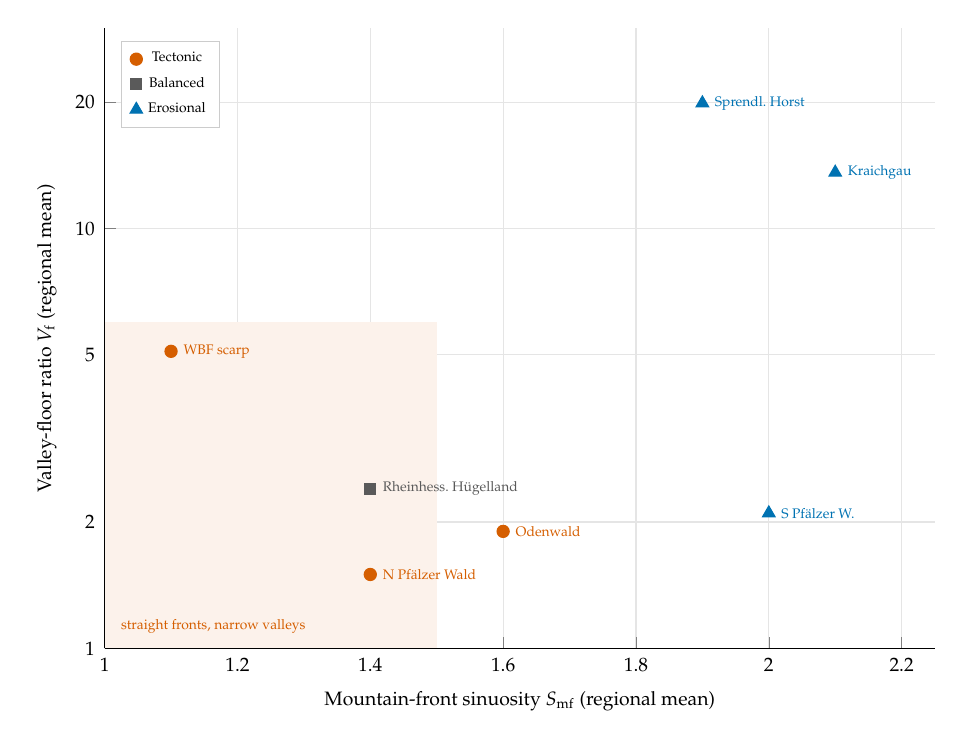
\begin{tikzpicture}
\begin{axis}[width=\columnwidth,height=0.78\columnwidth,
  xmin=1.0,xmax=2.25,ymode=log,ymin=1,ymax=30,
  xlabel={Mountain-front sinuosity $S_\mathrm{mf}$ (regional mean)},
  ylabel={Valley-floor ratio $V_\mathrm{f}$ (regional mean)},
  label style={font=\scriptsize},tick label style={font=\scriptsize},
  ytick={1,2,5,10,20},yticklabels={1,2,5,10,20},
  axis lines*=left,grid=major,grid style={gray!20},
  nodes near coords,point meta=explicit symbolic,
  every node near coord/.append style={font=\tiny,anchor=west,xshift=1pt},
  legend style={font=\tiny,at={(0.02,0.98)},anchor=north west,draw=gray!40}]
\fill[cB!8] (axis cs:1.0,1) rectangle (axis cs:1.5,6);
\addplot[only marks,mark=*,cB,mark size=2.2pt] coordinates {
  (1.1,5.1)[WBF scarp] (1.4,1.5)[N Pfälzer Wald] (1.6,1.9)[Odenwald]};
\addplot[only marks,mark=square*,cE,mark size=2pt] coordinates {
  (1.4,2.4)[Rheinhess.\ Hügelland]};
\addplot[only marks,mark=triangle*,cA,mark size=2.6pt] coordinates {
  (2.1,13.6)[Kraichgau] (1.9,19.9)[Sprendl.\ Horst] (2.0,2.1)[S Pfälzer W.]};
\legend{Tectonic,Balanced,Erosional}
\node[cB,font=\tiny,anchor=south west] at (axis cs:1.01,1.03) {straight fronts, narrow valleys};
\end{axis}
\end{tikzpicture}
\caption{Regional means of mountain-front sinuosity and valley-floor ratio along the northern URG
border faults, redrawn from Table 1 of \citet{PetersVanBalen2007}. Classes follow their interpretation.}
\label{fig:pvb}
\end{figure}

The indices separate the border faults into segments of higher and lower activity
(Table~\ref{tab:pvb}; Fig.~\ref{fig:pvb}). The WBF scarp, the northern Pfälzer Wald and the southern
Odenwald show straight fronts, narrow V-shaped or hanging valleys and sharp gradient changes where
streams cross the faults. The Kraichgau, the Sprendlinger Horst and the southern Pfälzer Wald show
embayed fronts, broad valleys and graded streams. Two comparisons make this result convincing. In
the Pfälzer Wald, the north and south are cut in the same Buntsandstein sandstone, yet their indices
differ strongly, so rock strength cannot explain the contrast. In the Odenwald, a straight front and
V-shaped valleys could be due to resistant granite, but the streams in the sandstone area south of
Heidelberg still show strong gradient changes. That segment also lies next to the deepest Quaternary
depocentre (about 380~m) and the highest shoulder topography (566~m).

Along the 20~km WBF scarp, longitudinal profiles change from almost concave in the south to convex in
the north, and the dry, hanging valleys are not adjusted to the 50--100~m height of the scarp. Because
fluvial erosion decreased sharply after about 15~ka, while slow faulting continued, the authors argue
that this tectonic landscape is largely a preserved Pleistocene feature rather than proof of present
activity. Intra-graben faults, though visible in scarps and in drainage orientation, produced no
measurable gradient change at a 20~m contour interval. This is a resolution limit rather than evidence
of inactivity.

\subsection{Western Rhenish shield: relative uplift age from $R_1$ and $S_\mathrm{r}$}
\label{sec:wrs}

\begin{table}[t]
\centering
\caption{Regional statistics of $R_1$ in the western Rhenish shield (from \citealp{Demoulin2011},
his Tables 2 and 3 and Fig. 3). Area 1: N Ardennes--N Eifel; area 2: central Ardennes--S Eifel--N
Hunsrück; area 3: S Ardennes--S Hunsrück--Saar-Nahe. Timing refers to the main uplift pulse.}
\label{tab:d11}
\scriptsize
\setlength{\tabcolsep}{3pt}
\begin{tabular}{@{}lccccc@{}}
\toprule
\textbf{Area} (uplift) & $n$ & $R_1$ (mean$\pm$s) & $S_\mathrm{r}$ & $b$ & $\rho$\\
\midrule
1 (rising now) & 28 & 0.99$\pm$0.73 & 0.51 & $-1.59$ & 0.93\\
2 ($\sim$0.8~Ma) & 35 & 1.03$\pm$0.45 & 0.35 & $-0.77$ & 0.88\\
3 (before 1~Ma) & 22 & 0.58$\pm$0.34 & 0.24 & $-0.54$ & 0.89\\
Whole area & 85 & 0.90$\pm$0.57 & 0.39 & $-1.07$ & 0.87\\
\bottomrule
\end{tabular}
\end{table}

\begin{figure}[t]
\centering
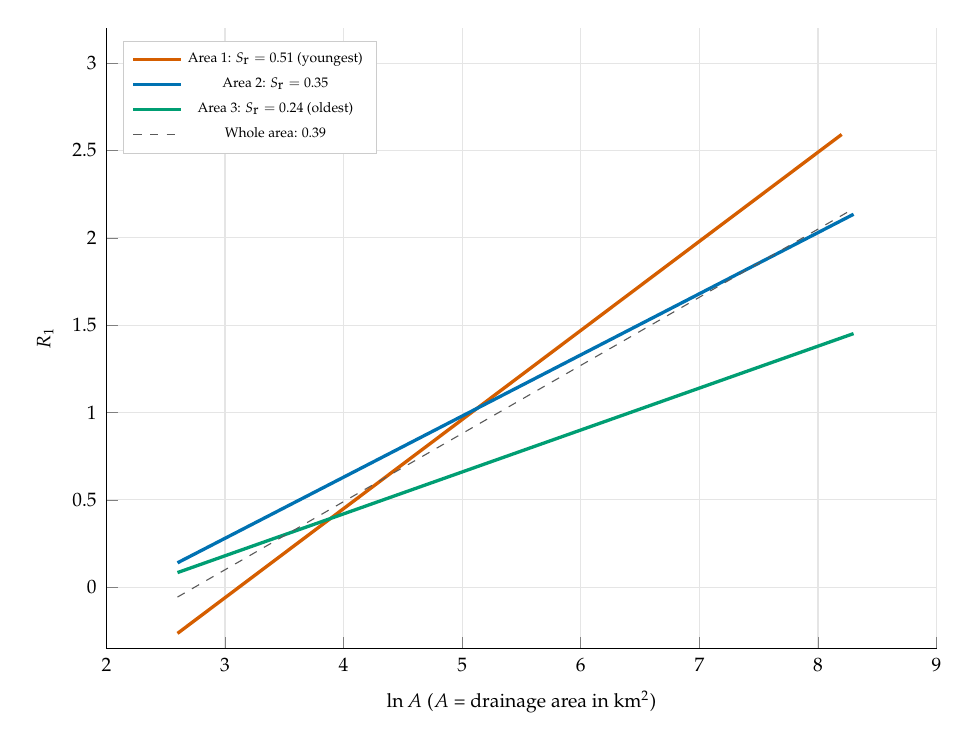
\begin{tikzpicture}
\begin{axis}[width=\columnwidth,height=0.78\columnwidth,
  xmin=2,xmax=9,ymin=-0.35,ymax=3.2,
  xlabel={$\ln A$ ($A$ = drainage area in km$^2$)},ylabel={$R_1$},
  label style={font=\scriptsize},tick label style={font=\scriptsize},
  axis lines*=left,grid=major,grid style={gray!20},
  legend style={font=\tiny,at={(0.02,0.98)},anchor=north west,draw=gray!40}]
\addplot[cB,very thick,domain=2.6:8.2] {0.51*x-1.59};
\addplot[cA,very thick,domain=2.6:8.3] {0.35*x-0.77};
\addplot[cC,very thick,domain=2.6:8.3] {0.24*x-0.54};
\addplot[cE,dashed,domain=2.6:8.3] {0.39*x-1.07};
\legend{Area 1: $S_\mathrm{r}=0.51$ (youngest),Area 2: $S_\mathrm{r}=0.35$,Area 3: $S_\mathrm{r}=0.24$ (oldest),Whole area: 0.39}
\end{axis}
\end{tikzpicture}
\caption{Regional regressions $R_1=S_\mathrm{r}\ln A+b$ for the three uplift-age areas of the western
Rhenish shield, drawn from the equations published by \citet{Demoulin2011}. Lines are plotted over the
basin-size range of the data set. The slope decreases with the age of uplift.}
\label{fig:d11}
\end{figure}

No single integral or difference index distinguished all three uplift-age areas
\citep{Demoulin2011}. Variation within each area was large, and most of it came from basin size. Once
$R_1$ was regressed on $\ln A$, however, the three areas separated clearly (Table~\ref{tab:d11};
Fig.~\ref{fig:d11}). Correlations were high ($\rho=0.88$--0.93), and covariance analysis showed that
the regional regressions differ in both position and slope. The slope $S_\mathrm{r}$ falls from 0.51 in
the currently rising north, to 0.35 in the area uplifted around 0.8~Ma, and to 0.24 in the area where uplift culminated before 1~Ma. The youngest area thus has about twice the slope of the oldest (derived ratio
2.1).

The interpretation rests on a simple model of how incision spreads. After a base-level fall, the trunk
stream cuts down first and fastest, so \Hr\ drops, $I_\mathrm{r}$ grows and $R_1$ rises within about
$10^4$--$10^5$ years. Over the following million years or so, incision spreads into the tributaries,
\Hn\ falls, $I_\mathrm{b}$ grows and $R_1$ declines; much later, slow hillslope denudation lowers \Hb\
and $R_1$ rises slightly again. Because knickpoints travel faster in larger basins, this sequence is
delayed in smaller ones, and the slope $S_\mathrm{r}$ therefore first steepens briefly and then flattens
with time. Single-river analyses along the Ourthe, Sûre and Nahe gave similar slopes but were disturbed
where a tributary drains a different uplift area, as at the Alzette and Glan confluences. Regional sets
of rivers were therefore preferred.

% =====================================================================
\section{Discussion}

\subsection{A shared logic: remove the dominant control, read the residual}

Despite their different indices, the three studies follow the same strategy. Each first identifies
the factor that controls most of the variation in its indices, removes or controls for it, and only
then looks for tectonics in what is left. In the Ardenne, this factor is hydraulics: the regression of
gradient on $\Hvm\cdot L/A$ explains about 70\% of the variance ($r^2\approx0.70$, derived), and tectonics is
read from the outliers. In the URG, it is lithology: regions are compared within the same rock type,
as in the northern and southern Pfälzer Wald, and lithological explanations are ruled out before
tectonic ones are accepted. In the Rhenish shield, it is basin size: $R_1$ is regressed on $\ln A$, and
the regional differences in slope are interpreted as time. In each case the tectonic signal is a
second-order effect, visible only after the first-order control is accounted for. This is perhaps the
most transferable lesson for other low-strain regions.

\subsection{Lithology and inherited relief}

All three studies treat lithology as the main source of false signals, but they deal with it in
different ways. \citet{Demoulin1998} discussed each river in its geological context and showed that
some steepened reaches follow rock boundaries, for example where the Hoyoux and Samson pass from
limestone onto Lower Devonian sandstone. \citet{PetersVanBalen2007} compared regions of similar rock
and accepted lithological explanations where these were sufficient, as for the Rhenish Massif streams.
\citet{Demoulin2011} formulated $R_1$ as a ratio so that lithological effects cancel, and chose an
area of fairly uniform slaty bedrock. A related problem is inheritance. Both the Condroz planation
surface in the Ardenne and the preserved Pleistocene scarps of the URG show that a landscape can
look tectonic long after the forcing has slowed or stopped. Morphometry alone therefore cannot prove
present-day activity; it needs independent evidence such as seismicity, geodesy or dated deformed
deposits.

\subsection{From where to when}

The three studies also show how the field has moved from mapping patterns to estimating timing.
Profile and front indices respond quickly, within about $10^4$--$10^5$ years (Fig.~\ref{fig:timescale}),
and are well suited to locating active structures or uplifting blocks. They say little about when the
movement started. The $R_1$--$S_\mathrm{r}$ approach adds a time dimension by using the fact that
different parts of a catchment respond at different speeds. The relation is still relative and
qualitative ($S_\mathrm{r}$ decreases with time since uplift), and \citet{Demoulin2011} noted that uplift
rate and uplift age cannot yet be fully separated. A later study by the same author extended the method
towards morphometric dating \citep{Demoulin2012}. Calibration against areas of known uplift age remains
the main step needed to make it quantitative.

\subsection{Consistency across the region}

Where the study areas overlap, the results agree. The NE Ardenne stands out in 1998 for its steep
gradients and for the rivers that plot above the hydraulic regression, and the same area belongs to the
youngest-uplift group with the highest $S_\mathrm{r}$ in 2011. Cosmogenic dating of the Younger Main
Terrace on the Meuse, Ourthe and Amblève supports this picture: post-terrace incision began about
0.73~Ma on the Meuse but only about 0.39 and 0.22~Ma on its Ardennian tributaries, consistent with an
erosion wave moving into the massif \citep{Rixhon2011}. Channel steepness and convexity in third-order
Ardenne catchments likewise show that these basins are still adjusting \citep{SougnezVanacker2011}. On
the eastern side, the high gradient indices of the Rhenish Massif streams in the URG study agree with
the stronger Quaternary uplift of the massif relative to the Mainz Basin, although
\citet{PetersVanBalen2007} attributed the local anomalies mainly to resistant rock.

\subsection{Data resolution and sample size}

Resolution affects each method differently. Map-based profiles with 2.5--5~m contours capture small
gradient changes but are laborious, which limits samples to tens of rivers. A 30~m DEM with 20~m
contours misses subtle steps on the graben floor, as \citet{PetersVanBalen2007} acknowledged. Integral
indices are less sensitive to resolution because errors partly cancel, which allowed
\citet{Demoulin2011} to use SRTM data. Modern high-resolution DEMs and lidar, together with automated
tools for stream-profile analysis \citep{SchwanghartScherler2014}, would now allow the detailed
approach of 1998 to be applied to hundreds of rivers. They would also allow the integral approach to be
tested against channel-steepness and $\chi$-based methods \citep{Wobus2006,PerronRoyden2013}.

\subsection{Strengths and limitations}

\begin{table*}[t]
\centering
\caption{Strengths, limitations and open questions of the three approaches.}
\label{tab:appraisal}
\footnotesize
\begin{tabularx}{\textwidth}{@{}P{2.4cm}LLL@{}}
\toprule
& \textbf{\citet{Demoulin1998}} & \textbf{\citet{PetersVanBalen2007}} & \textbf{\citet{Demoulin2011}}\\
\midrule
Strengths & Fine vertical detail from maps; field-validated bedload proxy; explicit separation of hydraulic and other controls & Combines long-term geological record with present landscape; natural lithological controls; segment-scale result & Large sample; lithology reduced by ratio form; adds relative timing; simple, reproducible workflow\\
Limitations & 24 rivers only; proxy not valid along a river; clusters do not match tectonic units; some anomalies unexplained & 20~m contours miss intra-graben signals; indices largely qualitative; tectonic landscape may be inherited & Coarse DEM; uplift age and rate not separated; relation $S_\mathrm{r}=f(t)$ uncalibrated; basin-shape outliers removed\\
Open question & Why do neighbouring NE Ardenne rivers differ so much? & Are intra-graben faults still active at the surface? & Can $S_\mathrm{r}$ be converted into absolute time?\\
\bottomrule
\end{tabularx}
\end{table*}

Table~\ref{tab:appraisal} summarises the strengths and weaknesses. None of the studies uses absolute
ages directly in its morphometric analysis, and all rely on terrace chronologies or geodetic data for
interpretation. The 1998 and 2007 results are mostly spatial, while the 2011 result is temporal but
only relative. Statistical treatment ranges from correlation and clustering to formal tests of
regression equality, and this progression is itself a useful development.

\subsection{Towards an integrated workflow}

\begin{figure}[t]
\centering
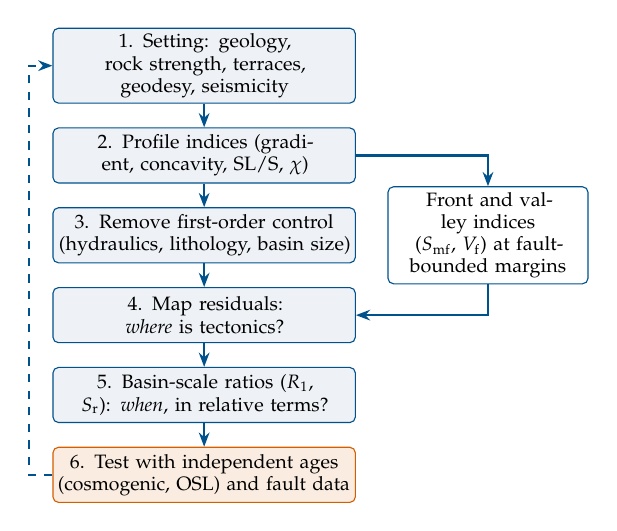
\begin{tikzpicture}[font=\scriptsize,
  box/.style={draw=accent,rounded corners=2pt,fill=boxgray,align=center,text width=37mm,minimum height=7mm,inner sep=2pt},
  arr/.style={-{Stealth[length=1.8mm]},thick,accent}]
  \node[box] (a) {1. Setting: geology, rock strength, terraces, geodesy, seismicity};
  \node[box,below=3mm of a] (b) {2. Profile indices (gradient, concavity, SL/S, $\chi$)};
  \node[box,below=3mm of b] (c) {3. Remove first-order control (hydraulics, lithology, basin size)};
  \node[box,below=3mm of c] (d) {4. Map residuals: \emph{where} is tectonics?};
  \node[box,below=3mm of d] (e) {5. Basin-scale ratios ($R_1$, $S_\mathrm{r}$): \emph{when}, in relative terms?};
  \node[box,below=3mm of e,fill=cB!12,draw=cB] (f) {6. Test with independent ages (cosmogenic, OSL) and fault data};
  \foreach \u/\v in {a/b,b/c,c/d,d/e,e/f}{\draw[arr] (\u)--(\v);}
  \node[box,right=4mm of c,text width=24mm,fill=white] (g) {Front and valley indices ($S_\mathrm{mf}$, $V_\mathrm{f}$) at fault-bounded margins};
  \draw[arr] (b.east) -| (g.north);
  \draw[arr] (g.south) |- (d.east);
  \draw[arr,dashed] (f.west) -- ++(-3mm,0) |- (a.west);
\end{tikzpicture}
\caption{Proposed multi-scale workflow combining the strengths of the three reviewed approaches.}
\label{fig:workflow}
\end{figure}

Fig.~\ref{fig:workflow} proposes a workflow that combines the strengths of the three approaches. The
geological setting is described first, so that lithological and inherited features are known in
advance. Profile indices are then computed for many rivers from a high-resolution DEM, and the
dominant non-tectonic control is modelled and removed. Residuals are mapped to show where tectonic
influence is likely. Where faults bound the relief, front and valley indices are added. Basin-scale
ratios such as $R_1$ are then used to estimate relative timing. Finally, the results are tested against
independent ages and fault data. Composite indices that combine several measures, such as the index
of relative active tectonics of \citet{ElHamdouni2008}, could serve as a summary at the regional scale.

% =====================================================================
\section{Future research directions}

\begin{enumerate}
  \item \textbf{Calibrating $S_\mathrm{r}$.} Apply the $R_1$--$S_\mathrm{r}$ method in regions of known uplift
        age and rate, ideally with cosmogenic or terrace chronologies, to turn the relative scale into
        an absolute one.
  \item \textbf{Separating uplift rate from age.} Test regions where rate varies but timing is similar,
        and vice versa, as suggested by \citet{Demoulin2011}.
  \item \textbf{High-resolution re-analysis.} Re-examine the Ardenne profiles and the URG
        intra-graben faults with lidar-based DEMs and contour intervals well below 20~m.
  \item \textbf{Linking with $\chi$ and steepness.} Compare profile, integral and $\chi$-based indices on
        the same rivers to test which best separates tectonic and lithological signals.
  \item \textbf{Quantifying rock strength.} Replace qualitative lithological classes with measured rock
        strength or erodibility, so that lithology can be removed statistically.
  \item \textbf{Joint use with geodesy and seismology.} Compare morphometric anomalies with modern
        GNSS velocities and seismicity to separate active from inherited landscapes.
\end{enumerate}

% =====================================================================
\section{Conclusions}

The three studies reviewed here show that tectonic signals can be recovered from fluvial landscapes even
where deformation is very slow, provided that the dominant non-tectonic controls are dealt with first.
In the Ardenne, profile parameters and a map-based bedload proxy identify current uplift of the NE
massif, relative subsidence around Namur and a Late Pleistocene base-level fall in the Famenne. In the
northern Upper Rhine Graben, the combined use of gradient, front and valley indices separates active
segments of the border faults (WBF scarp, northern Pfälzer Wald, southern Odenwald) from segments
dominated by erosion. In the western Rhenish shield, the slope $S_\mathrm{r}$ of the relation between
$R_1$ and basin size orders three areas by uplift age, from 0.51 in the youngest to 0.24 in the oldest.

Profile and front indices tell us \emph{where} tectonics acts; basin-scale ratios begin to tell us
\emph{when}. All of these methods remain sensitive to lithology, inheritance and data resolution, and
none yet gives absolute ages. Combining them within a single, multi-scale workflow that is tested
against independent chronologies offers the best route to a reliable reading of tectonics from rivers in
low-strain intraplate regions.

% =====================================================================
\section*{Acknowledgements}
\noindent [Add acknowledgements and funding details here.]

\section*{Declarations}
\noindent\textit{Competing interests:} The authors declare no competing interests.\\
\textit{Data availability:} All values discussed are taken from the published sources cited; the
figures were redrawn from these values.

% =====================================================================
\begin{thebibliography}{99}
\setlength{\itemsep}{1pt}
\footnotesize

\bibitem[Bull and McFadden(1977)]{BullMcFadden1977}
Bull, W.B., McFadden, L.D., 1977. Tectonic geomorphology north and south of the Garlock fault,
California. In: Doehring, D.O. (Ed.), Geomorphology in Arid Regions. Proceedings of the 8th Annual
Geomorphology Symposium. State University of New York, Binghamton, pp. 115--138.

\bibitem[Burbank and Anderson(2001)]{BurbankAnderson2001}
Burbank, D.W., Anderson, R.S., 2001. Tectonic Geomorphology. Blackwell Science, Oxford.

\bibitem[Demoulin(1998)]{Demoulin1998}
Demoulin, A., 1998. Testing the tectonic significance of some parameters of longitudinal river
profiles: the case of the Ardenne (Belgium, NW Europe). Geomorphology 24, 189--208.

\bibitem[Demoulin(2011)]{Demoulin2011}
Demoulin, A., 2011. Basin and river profile morphometry: a new index with a high potential for
relative dating of tectonic uplift. Geomorphology 126, 97--107.

\bibitem[Demoulin(2012)]{Demoulin2012}
Demoulin, A., 2012. Morphometric dating of the fluvial landscape response to a tectonic perturbation.
Geophysical Research Letters 39. \url{https://doi.org/10.1029/2012GL052201}

\bibitem[Demoulin and Hallot(2009)]{DemoulinHallot2009}
Demoulin, A., Hallot, E., 2009. Shape and amount of the Quaternary uplift of the western Rhenish
shield and the Ardennes (western Europe). Tectonophysics 474, 696--708.

\bibitem[El Hamdouni et~al.(2008)]{ElHamdouni2008}
El Hamdouni, R., Irigaray, C., Fernández, T., Chacón, J., Keller, E.A., 2008. Assessment of relative
active tectonics, southwest border of the Sierra Nevada (southern Spain). Geomorphology 96, 150--173.

\bibitem[Hack(1973)]{Hack1973}
Hack, J.T., 1973. Stream-profile analysis and stream-gradient index. Journal of Research of the U.S.
Geological Survey 1, 421--429.

\bibitem[Keller and Pinter(2002)]{KellerPinter2002}
Keller, E.A., Pinter, N., 2002. Active Tectonics: Earthquakes, Uplift, and Landscape, 2nd edn.
Prentice Hall, Upper Saddle River, NJ.

\bibitem[Kirby and Whipple(2012)]{KirbyWhipple2012}
Kirby, E., Whipple, K.X., 2012. Expression of active tectonics in erosional landscapes. Journal of
Structural Geology 44, 54--75.

\bibitem[Merritts and Vincent(1989)]{MerrittsVincent1989}
Merritts, D., Vincent, K.R., 1989. Geomorphic response of coastal streams to low, intermediate, and
high rates of uplift, Mendocino triple junction region, northern California. Geological Society of
America Bulletin 101, 1373--1388.

\bibitem[Perron and Royden(2013)]{PerronRoyden2013}
Perron, J.T., Royden, L., 2013. An integral approach to bedrock river profile analysis. Earth Surface
Processes and Landforms 38, 570--576.

\bibitem[Peters and Van Balen(2007)]{PetersVanBalen2007}
Peters, G., Van Balen, R.T., 2007. Tectonic geomorphology of the northern Upper Rhine Graben, Germany.
Global and Planetary Change 58, 310--334.

\bibitem[Rixhon et~al.(2011)]{Rixhon2011}
Rixhon, G., Braucher, R., Bourlès, D., Siame, L., Bovy, B., Demoulin, A., 2011. Quaternary river
incision in NE Ardennes (Belgium) -- insights from $^{10}$Be/$^{26}$Al dating of river terraces.
Quaternary Geochronology 6, 273--284.

\bibitem[Schwanghart and Scherler(2014)]{SchwanghartScherler2014}
Schwanghart, W., Scherler, D., 2014. TopoToolbox 2 -- MATLAB-based software for topographic analysis
and modeling in Earth surface sciences. Earth Surface Dynamics 2, 1--7.

\bibitem[Silva et~al.(2003)]{Silva2003}
Silva, P.G., Goy, J.L., Zazo, C., Bardají, T., 2003. Fault-generated mountain fronts in southeast
Spain: geomorphologic assessment of tectonic and seismic activity. Geomorphology 50, 203--225.

\bibitem[Sougnez and Vanacker(2011)]{SougnezVanacker2011}
Sougnez, N., Vanacker, V., 2011. The topographic signature of Quaternary tectonic uplift in the
Ardennes massif (Western Europe). Hydrology and Earth System Sciences 15, 1095--1107.

\bibitem[Strahler(1952)]{Strahler1952}
Strahler, A.N., 1952. Hypsometric (area--altitude) analysis of erosional topography. Geological
Society of America Bulletin 63, 1117--1142.

\bibitem[Van Balen et~al.(2000)]{VanBalen2000}
Van Balen, R.T., Houtgast, R.F., Van der Wateren, F.M., Vandenberghe, J., Bogaart, P.W., 2000.
Sediment budget and tectonic evolution of the Meuse catchment in the Ardennes and the Roer Valley Rift
System. Global and Planetary Change 27, 113--129.

\bibitem[Wobus et~al.(2006)]{Wobus2006}
Wobus, C., Whipple, K.X., Kirby, E., Snyder, N., Johnson, J., Spyropolou, K., Crosby, B., Sheehan, D.,
2006. Tectonics from topography: procedures, promise, and pitfalls. In: Willett, S.D., Hovius, N.,
Brandon, M.T., Fisher, D.M. (Eds.), Tectonics, Climate, and Landscape Evolution. Geological Society of
America Special Paper 398, pp. 55--74.

\end{thebibliography}

\end{document}
